\chapter{Data}
\label{chap:data}
% \thispagestyle{fancy}
This chapter discusses the datasets used in the thesis, as well as the processing steps to make the data more learnable. The main dataset used in the thesis is \textit{Human3.6M}: Large Scale Datasets and Predictive Methods for 3D Human Sensing in Natural Environments \cite{H3.6}. Most of the related works benchmark their methods on Human3.6M and it also is freely accessible to academics on request. For further evaluation of model performance in the wild, outdoor datasets that do not have 3D ground truth such as \textit{3DPW}: 3D Poses in the Wild \cite{3dpw} would be used.

\begin{figure}[h]
    \centering
    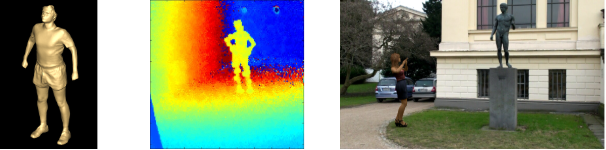
\includegraphics[width=\textwidth]{figures/h36/modlities.png}
    \caption{Full body model, depth from time of flight and mixed reality in Human3.6M dataset}
    \label{fig:h36_modality}
\end{figure}

\section{Human3.6M}
Human3.6M is a large scale indoor dataset with 3.6 million human poses collected with 4 cameras at different angles using a highly accurate maker-based \ac{mocap} system. The dataset constitutes 15 diverse motion and actions such as eating, sitting, walking in various everyday scenarios such as, a hand in the pocket, talking over the phone, walking a dog etc. These actions are performed by 11 professional actors wearing a variety of realistic clothing. The datasets provides synchronised 2D and 3D data including full-body scans as shown in figure[\ref{fig:h36_modality}]. It also includes mixed-reality test data created using animated human models to cover huge variations of background, clothing, illumination, occlusion and camera angles.

% TODO -- Add things related to 3D projection, depth ambiguity, rigid body alignment
\section{3D Geometry}
\lipsum[1-4] %FIXME
\subsection{Perspective projection}
\lipsum[1] %FIXME
\subsection{Depth Ambiguity and Camera Modeling}
\lipsum[1] %FIXME
\subsection{Procrustes Alignment}
\lipsum[1-4] %FIXME

\section{Processing}

The methods explored by this thesis would require only images, 2D and 3D human pose from the dataset. The following are the pre-processing steps for the 2D and 3D poses.

The 3D pose in the dataset that are obtained from the marker-based \ac{mocap} are in a global reference frame. These poses using the camera parameters, are transformed into the camera coordinate frame. For the task of predicting 3D pose from either images or 2D pose, it is unrealistic to directly estimate all the joints of the pose in a global frame. So the first step of processing would be to zero the pose w.r.t the root joint say, Pelvis. As the root is always zero, we remove it so we do not have to learn the constant joint. Removing Pelvis, 16 out of the 17 joints or keypoints remain. The 3D pose is then normalized with the mean and standard deviation of the entire training and validation poses respectively.

\begin{figure}[h]
    \centering
    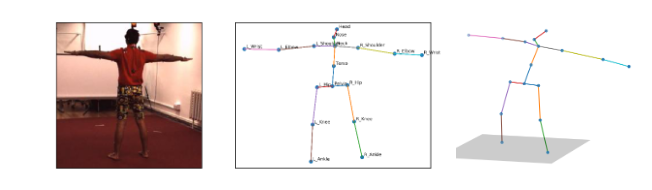
\includegraphics[width=\textwidth]{figures/h36poses.png}
    \caption{Human3.6M Pose Sample}
    \label{fig:h36_poses}
\end{figure}

The 2D pose which is obtained from the 3D pose, is also in the camera coordinate frame. The 2D pose is not zeroed as the cameras used to capture the data are not orthogonal but are perspective cameras. Zeroing the root of the 2D would eliminate the perspective information that could be important to estimate the 3D pose. The experiments to test the importance of that information is yet to be done. The root of the 2D pose is however removed to remain consistent with the 3D pose. Similar to the 3D, the 2D pose is also normalized. An image sample from the dataset with its corresponding 2D and 3D pose before normalization are illustrated in the figure[\ref{fig:h36_poses}].

% TODO update - experiments are yet to be done
% TODO link MPJPE to its explanation in other chapter or sections

The estimated poses from the networks that are trained on normalized poses are denormalized to the original scale using the same mean and standard deviation. This postprocessing step is required for getting the distance between prediction and ground truth keypoints in understandable units like millimeters. It is also necessary to denormalize for visualizing the poses, as poses normalized over all the keypoints appear heavily skewed and distorted.


